
\chapter{Aplicaciones}

\section{Librerías utilizadas}

Este proyecto ha sido implementado en el lenguaje de programación C++ \cite{cplusplus} haciendo extenso uso de librerías \textit{open source}. En primer lugar, se presentan las librerías utilizadas, y de forma seguida, se describe brevemente cómo se aplicaron en este trabajo.

\begin{itemize}

\item OpenNI. (Open Natural Interaction) OpenNI es un conjunto de API’s escritas en C/C++, \textit{open source}, distribuidas bajo la licencia LGPL. Las API's (\textit{Application Programming Interface}) de OpenNI incluyen interfaces de acceso a las cámaras RGB, de rango, micrófonos, así como componentes de más alto nivel como detección de gestos, \textit{skeleton tracking}, etc.
Son soportadas por la organización sin ánimo de lucro, OpenNI, liderada por la industria y centrada en la mejora de los dispositivos de interacción de forma natural. Uno de sus socios principales es PrimeSense, empresa responsable de la tecnología que utiliza el sensor Kinect. 

\item OpenCV. (Open Source Computer Vision Library) Librería escrita en C/C++, multiplataforma y \textit{open source}, distribuida bajo la licencia BSD. La librería OpenCV incluye algoritmos de procesamiento de imágenes y de visión por computadora como emparejamiento de características, visión estéreo, detección de objetos, etc.

\item PCL. (Point Cloud Library) Librería escrita en C++, multiplataforma y \textit{open source}, distribuida bajo la licencia BSD. La librería PCL incluye algoritmos para el procesamiento de nubes de puntos n-dimensionales y geometría 3D, así como métodos específicos para realizar filtrado, segmentación, detección de características, reconstrucción 3D, etc.

\item Eigen. Librería escrita en C++, open source, distribuida bajo la licencia LGPL. La librería incluye métodos de álgebra lineal; como operaciones sobre matrices y vectores, métodos numéricos de resolución de sistemas lineales, etc.

\item FLANN. (Fast Library for Approximate Nearest Neighbors) Librería escrita en C++, multiplataforma y \textit{open source}, distribuida bajo la licencia BSD. La librería FLANN incluye algoritmos para realizar búsquedas de los vecinos más cercanos en espacios de elevada dimensión.

\item Boost. Conjunto de librerías escritas en C++, multiplataforma y \textit{open source}, distribuidas bajo la licencia Boost Software License. Las librerías Boost incluyen métodos para álgebra lineal, \textit{multithreading}, \textit{smart pointers}, procesamiento de imágenes, test unitarios, etc.

\item VTK. (Visualization Toolkit) Librería escrita en C++, multiplataforma y \textit{open source}, distribuida bajo la licencia BSD. La librería incluye una amplia variedad de algoritmos para visualización de texturas, volúmenes, etc.

\end{itemize}

Conceptualmente, el proyecto puede dividirse en varios bloques de software, que se describen a continuación :
\begin{itemize}

\item Captura y almacenamiento de datos: se utiliza el formato PCD (\textit{Point Cloud Data}), propio de PCL, para el almacenamiento de nubes de puntos. Para capturar los datos provistos por la Kinect, se utiliza un API provista por PCL, que por debajo interactúa con el driver OpenNI para acceder al dispositivo. Se aprovecha el modo de captura sincronizada de frames RGB y de profundidad (implementado en OpenNI) para integrar la información en nubes de puntos RGB-D.

\item Procesamiento de imágenes 2D: OpenCV provee algoritmos para la detección de características 2D, entre ellos destacan las implementaciones de ORB y SURF, y procedimientos para determinar correspondencias con descriptores binarios y reales.

\item Procesamiento de nubes de puntos 3D: PCL contribuye en múltiples etapas en el proceso de registración. Provee la aproximación de la pose utilizando SVD y soporta varias versiones de ICP para el refinamiento de la transformación rígida. Contiene una implementación genérica de RANSAC, que puede ser instanciada con el modelo de transformación rígida para eliminar outliers 3D. En el terreno de \textit{GraphSLAM}, brinda una estructura para construir el grafo de poses e implementa el algoritmo para aplicar la optimización global basado en el enfoque de Lu y Milios. Por último, cabe destacar que PCL cuenta con varios métodos de filtrado de puntos, entre ellos la técnica de filtrado estadístico presentada en la sección \ref{sec:filtrado-estadistico-de-inconsistencias}.

\item Visualización de datos: se utiliza el \textit{framework} de visualización de nubes de puntos 3D provisto por PCL, construido encima de la librería VTK.

\item Librerías auxiliares de propósito específico: PCL y OpenCV implementan sus algoritmos apoyados en otras librerías \textit{open source} que llevan a cabo tareas más específicas. Para manejar vectores y transformaciones (representadas por matrices) PCL utiliza Eigen, que soporta operaciones de álgebra lineal. Boost se encarga del manejo automático de la memoria en PCL y contiene estructuras para construir el grafo de poses. Tanto OpenCV como PCL se apoyan en FLANN para realizar búsquedas de vecinos más cercanos, el primero en espacios de grandes dimensiones, mientras que el último principalmente en 3D.

\end{itemize}

\section{Aplicaciones}

Este proyecto se ha implementado y probado sobre el sistema operativo Ubuntu \cite{ubuntu} y requiere de las librerías \textit{open source} citadas en la sección anterior. El sistema se divide en dos componentes, la aplicación \textit{ModelMapper} que genera un mapa 3D (en sistema modelo) a partir de la condición de erosión del modelo físico y la aplicación \textit{RealWorldConverter} que filtra inconsistencias y retorna un mapa 3D convertido a sistema prototipo. Para simplificar la implementación, se utiliza una interfaz de líneas de comandos \cite{wiki-linea-de-comandos}, estándar en sistemas GNU/Linux \cite{wiki-gnu-linux}.

\subsection{\textit{ModelMapper}}
\label{sec:model-mapper}
La finalidad de esta aplicación es generar un mapa 3D de una zona de interés del modelo físico sobre el que se trabaja. Toma nubes de puntos RGB-D como entrada y devuelve las nubes de puntos alineadas en el sistema de coordenadas modelo (apartado \ref{sec:conversion-mapa3D-prototipo}) utilizando la técnica de registración presentada en \ref{sec:descripcion-general-registracion}. \\
Al finalizar la registración, las nubes de puntos alineadas se almacenan en un directorio llamado \textit{registration}, creado (automáticamente) dentro de un directorio \textit{base} especificado por el usuario. La ruta del directorio \textit{base} se ingresa a través de la opción --output-dir (requerimiento obligatorio). \\
La opción --backup habilitar el guardado de las nubes de puntos de entrada (a medida que se van procesando) en un directorio llamado \textit{backup}, creado (automáticamente) dentro del directorio \textit{base}. Esta opción se encuentra deshabilitada por default.\\
Se plantearon dos métodos para ingresar las nubes de puntos, que se pueden seleccionar utilizando la opción --mode.
Los valores aceptados son \textsl{camera} (modo cámara) y \textsl{files} (modo archivos). Por default se trabaja en modo cámara.
\begin{itemize}

\item Modo cámara: los frames RGB-D son capturados directamente desde el sensor Kinect y registrados inmediatamente. En la figura \ref{fig:modelmapper-camera-mode}, se muestra la pantalla observada en este modo. A la izquierda, se visualiza la última nube de puntos registrada. A la derecha, se observa el estado parcial de la registración. Se requiere presionar la tecla \textit{espacio} para procesar un nuevo frame. Presionando la tecla \textit{p} se finaliza la registración.

\item Modo archivos: los frames RGB-D son obtenidos desde el sistema de archivos. Este modo está pensado para correr el proceso de registración con frames capturados con el modo cámara (con la opción --backup habilitada) y probar diferentes parametros para el algoritmo de registración (los cuales se explicaran en los párrafos siguientes). Se requiere ingresar la opción --input-dir seguida del directorio \textit{base} que contiene la carpeta \textit{backup}. Este modo es completamente automático, es decir, que no requiere interacción alguna por parte del usuario (nota: no se muestra el visualizador con las nubes de puntos).

\end{itemize}

\begin{figure}[ht]
\centering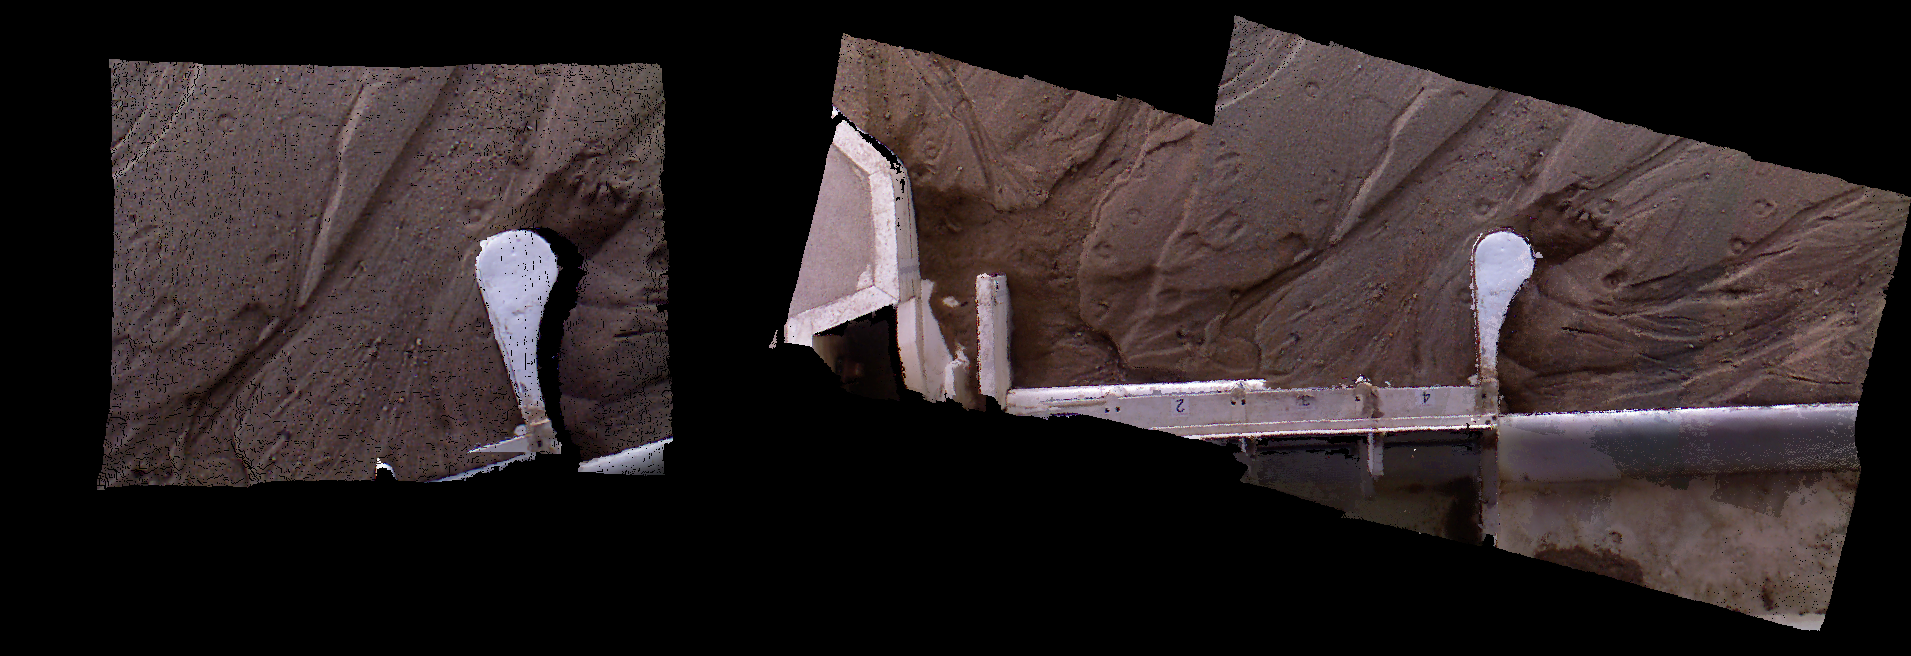
\includegraphics[width=\imsizeL]
{modelmapper-camera-mode}
\caption[ModelMapper en modo cámara]
{ModelMapper en modo cámara. Izquierda: última nube de puntos registrada. Derecha: estado parcial de la registración.}
\label{fig:modelmapper-camera-mode}
\end{figure}

A continuación, se lista una serie de parametros del algoritmo de registración que pueden ser modificados desde la interfaz de líneas de comandos:

\begin{itemize}

\item Opción --features: tipo de algoritmo para extraer características visuales. Posibles valores: \textsl{surf, orb}. Default: \textsl{orb}. Detalles en el apartado \ref{sec:features}.

\item Opción --min-num-inliers: mínima cantidad de correspondencias correctas para considerar que la odometría fue medida exitosamente. Default: 45. Detalles en el apartado \textit{front-end} de \textit{GraphSLAM} \ref{sec:slam-frontend}.	

\item Opción --min-num-extra-inliers: mínima cantidad de correspondencias correctas para la detección de bucles en un mapa. Default: 25. Detalles en el apartado \textit{front-end} de \textit{GraphSLAM} \ref{sec:slam-frontend}.

\item Opción --extra-edges: Máxima cantidad de aristas con las que se puede extender el grafo de poses en la etapa de detección de bucles. Default: 2. Detalles en el apartado \textit{front-end} de \textit{GraphSLAM} \ref{sec:slam-frontend}.

\end{itemize}

Se destaca que esta aplicación explícitamente almacena el mapa 3D dividido en varios archivos PCD. 

\subsection{\textit{RealWorldConverter}}
 
Esta aplicación cumple dos tareas, eliminar posibles inconsistencias que afectan al mapa 3D generado con ModelMapper utilizando la técnica de filtrado estadístico (explicada en la sección \ref{sec:filtrado-estadistico-de-inconsistencias}) y generar un mapa 3D en sistema prototipo (presentado en la sección \ref{sec:conversion-mapa3D-prototipo}) para que pueda ser utilizado en estudios de la erosión.

ModelMapper almacena el mapa 3D dividido en diferentes archivos debido a que RealWorldConverter brinda la posibilidad de seleccionar un subconjunto del total de nubes de puntos, con la finalidad de crear un mapa más liviano o de una zona específica. 

Los parámetros obligatorios a ingresar en esta aplicación son:

\begin{itemize}
\item Opción --input $ cloud_{1}, ..., cloud_{n} $: lista de nubes de puntos de entrada.

\item Opción --output cloud\_final.pcd: path para almacenar el mapa 3D filtrado en sistema prototipo.

\item Opción --scale s: factor de escala.

\item Opción --real\_base r: cota de referencia en prototipo.

\end{itemize}

Para ingresar la cota de referencia en modelo hay dos posibilidades: 
\begin{itemize}

\item Ingresar la opción --model\_base m, donde m es valor de la cota.

\item Si no se ingresó la opción anterior, se visualiza el mapa 3D en sistema modelo y se debe seleccionar un punto 3D (con la combinación shift + click derecho) para aplicar su altitud como cota de referencia en modelo.

\end{itemize}

% Hay dos parametros opcionales para configurar el algoritmo de filtrado estadístico:
% AGREGAR PARAMETROS

